% -*-LaTeX-*- 
% derived from file acl08.tex
%

\documentclass[11pt]{article}
\usepackage{acl08}
\usepackage{times}
\usepackage{latexsym}
\usepackage{amsmath}
\usepackage{dcolumn}
\usepackage{url}
\usepackage{comment}
\usepackage{graphicx}
\usepackage{qtree}
\setlength\titlebox{6.5cm}    % Expanding the titlebox

%\newcommand{\blindthis}[1]{#1}
\newcommand{\blindthis}[1]{}

\newcolumntype{d}{D{.}{.}{3}}
\DeclareMathOperator*{\corr}{corr}

\title{Automatic Syntactic MT Evaluation with Expected Dependency
  Pair Match\protect\blindthis{\Thanks{Thanks to Kevin Knight for providing data for
    earlier revisions of this research.}}}

\author{\blindthis{
    Jeremy G. Kahn \and Mari Ostendorf \\
    Signal, Speech, and Language Interpretation Laboratory \\
    University of Washington \\
    Seattle, WA 98195, USA\\
    {\tt \{jgk,mo\}@ssli.ee.washington.edu}
    \And
    Brian Roark\\
    OGI
  }
}
\date{}


\newcommand{\headlabel}[2]{\ensuremath{\underset{\textrm{#2}}{\textrm{#1}}}}
\newcommand{\arclabel}[1]{\ensuremath{\stackrel{#1}{\to}}}
\newcommand{\DPM}[1]{\ensuremath{\mathrm{DPM}_{#1}}}
\newcommand{\DPMempty}{\ensuremath{\DPM{}}}
% \newcommand{\EDPM}[2]{
%   \DPM{ E^{#2} \left[ #1 \right] }
% }
\newcommand{\EDPM}[2]{\ensuremath{\DPM{#1}{#2}}}
\newcommand{\mDPM}[2]{\ensuremath{\DPM{#1}{0}}}
\newcommand{\bDPM}[1]{\ensuremath{\mathrm{b}\DPM{#1}}}
\newcommand{\myEDPM}[0]{\ensuremath{\mathrm{EDPM}}}
\newcommand{\BoNG}[1]{\ensuremath{\textrm{bag-of-ngrams}(#1)}}
% \newcommand{\BoNG}[1]{
%   \ensuremath{F_\cup \left(n_1^{#1}  \textrm{-gram} \right)
%   }}
\newcommand{\bBoNG}[1]{\ensuremath{\textrm{av-bags-of-ngrams}(#1)}}
% \newcommand{\bBoNG}[1]{
%   \ensuremath{F_\forall \left(
%       n_1^#1\textrm{-gram}
%     \right)}}

\newcommand{\ngram}[0]{\ensuremath{n\textrm{-gram}}}
\newcommand{\precision}[0]{\ensuremath{\textrm{Precision}}}
\newcommand{\recall}[0]{\ensuremath{\textrm{Recall}}}

\begin{document}
\maketitle
\begin{abstract}
  % TO DO: cut further per M.O. comments?
  Previous work on dependency-based machine translation evaluation
  % \cite{owczarzak07labelleddepseval} 
  has shown that an LFG-based F-measure of labeled partial
  dependencies over an $n$-best list %(\textbf{d\_$n$\_var})
  has improved correlation with human judgments of fluency and
  adequacy as compared to BLEU %\cite{papineni02bleu}
  and TER. %\cite{snover06ter}
  Inspired by \textsc{SParseval}, % \cite{roark06:sparseval}
  we demonstrate that a statistical syntactic parser based on PCFGs
  % \cite{charniak-johnson:2005:ACL} 
  may be used in place of the LFG dependencies, and we explore
  variations on other aspects of the %\textbf{d\_$n$\_var}
  dependency-matching method. We
  find that separating the match quality into different bins, as in
  BLEU, does \emph{not} improve correlations with human judgments, but
  that including $n>1$ parses helps, especially if one incorporates
  probabilistic weights from the parser.  Additionally, we find that
  matching simple words (along with partial-dependencies) further improves
  correlations with human judgments. % beyond \textbf{d\_$n$\_var}.

  From these results, we design a new scoring metric ``Expected
  Dependency Pair Match'' (\myEDPM), and 
%   explore \myEDPM's quality
%   with respect to the GALE % \cite{olive06gale}
%   2.5 evaluations corpus.  We 
  demonstrate that $\Delta$\myEDPM{} is superior to $\Delta$BLEU and
  $\Delta$TER as a per-document and per-sentence predictor of
  $\Delta$HTER.
% , and is superior to $\Delta$TER in
%   the written contexts (newswire and web text).
\end{abstract}

\section{Introduction}

Machine translation (MT) evaluation is a challenge for research
because the space of good translations is large, and two equally good
translations may appear to be quite different at first glance. 
%
The challenges of choosing among translations are compounded when this
evaluation is done automatically.
%
Human evaluation, however, is both time-consuming and difficult, so
research % since at least \cite{papineni02bleu}
has turned increasingly towards automatic measures of translation
quality, usually by comparing the system translation to one or more
reference (human) translations.
%
Automatic measures of this kind (e.g.\ BLEU \cite{papineni02bleu}) not
only provide a well-defined evaluation standard but are also required
for training on error criteria, e.g.\ with minimum error rate training
\cite{och03mert}.

The most popular evaluation measures (BLEU and related measure
NIST \cite{doddington02nist}) are based on $n$-gram precision.  More
recent research has found that these measures may not accurately track
translation quality both empirically \cite{charniak03syntaxlmmt} and
theoretically \cite{callisonburch06bleuproblems}.

% \subsection{Syntactic machine translation evaluation}
One direction to look for improving metrics is to try to model
acceptable variation, whether word-choice (e.g.\ METEOR
\cite{banerjee05meteor}, which does progressively more forgiving
word matching) or by modeling syntactic information
\cite{liu05syntaxformteval,owczarzak07labelleddepseval}.  
\newcite{owczarzak07labelleddepseval} explore the correlation of
their measure \textbf{d} and \textbf{d\_var} with human judgment, and
report substantial improvements relative to the popular measures BLEU
and TER \cite{snover06ter}.  
%
Keeping to the syntactic approach, the work here follows and extends
the labelled-dependency match version of \textsc{SParseval}
\cite{roark06:sparseval} and the \textbf{d}/\textbf{d\_var}
\cite{owczarzak07labelleddepseval} measures, all of which evaluate
hypothesis-reference similarity with an $F$ measure over fragments of
a labelled dependency structure.  
%
The measures requiring dependency structure have generated that structure by a
PCFG with deterministic head-finding
\cite{liu05syntaxformteval,roark06:sparseval} or by extracting the
semantic dependencies from an LFG parser
(\newcite{cahill04lfg} in \newcite{owczarzak07labelleddepseval}).
In this work, we extend the dependency-scoring strategies of
\newcite{owczarzak07labelleddepseval} but do so with a
widely used and publically available PCFG parser and
deterministic head-finding rules instead of an LFG system.

% Prior work with
% \textsc{SParseval} (which has generally been used for
% speech-recognition evaluation rather than MT) has generally used a PCFG and the \textbf{d}
% measure is the source of the dependency graph; the latter uses an LFG
% parser \cite{cahill04lfg} while the former uses a PCFG parse and a
% deterministic head-finding strategy.

%% TO DO: MO: SParseval has multiple versions, only one of which uses the
%% head-finding structure. I don't think that SParseval *requires* the
%% use of a PCFG which is the model.  It simply requires a certain
%% form of the resulting parse. 

%% Comparing SParseval and d might make
%% sense if d has been used for parsing as well as MT, but then you
%% should be citing the parsing paper. If not, you can distinguish the
%% LFG and PCFG aspects of the two approaches work, but should
%% separate that from SParseval and d/dvar. 

%% In the list of diffs, you
%% might also talk about looking at correlation with two types of
%% human assessments: FL & Ad and HTER.

%\subsection{Evaluation of MT metrics}
These measures have been evaluated in a number of ways.  Some
\cite{banerjee05meteor,liu05syntaxformteval,owczarzak07labelleddepseval}
have evaluated their success by comparing the measure to human
judgments of fluency and adequacy.  In other work,
e.g. \newcite{snover06ter}, 
%and the GALE translation and summarization project
measures are evaluated by comparison to
HTER, a distance to a human-revised reference that uses wording closer
to the MT system choices (keeping the original meaning) that
%\emph{post hoc} human-targeted reference, which
is intended to measure the post-editing work required after
translation.  In this paper, we pursue both kinds of evaluation.

The remainder of this work is as follows. In section~\ref{sec:dpm}, we
define a family of measures \DPM{} that include \textsc{SParseval} and
\textbf{d}/\textbf{d\_var} measures and describe our strategy for
extracting labelled dependencies. In section~\ref{sec:facorr}, we
explore a selection of variants of that family with human judgments
over the Multiple Translation Chinese corpus
\cite{LDC03MTC2,LDC06MTC4}. We explore questions of dependency-graph
decomposition, binning choices, using multiple parses, and
parse-confidence and select a member of that family as a new best
measure \myEDPM{} that we believe to be a superior representative of
the \DPM{} family.  In section~\ref{sec:hter}, we explore \myEDPM{}'s
ability to predict changes in a human-generated score (HTER) over a
corpus of hypothesis translations in the GALE 2.5 \cite{darpa08gale}
% \cite{olive06gale}
% TO DO: MO: find better citation for GALE (cf. NIST web site or
% Google)
evaluation. In section~\ref{sec:conclusion}, we discuss future work
and conclude.

% Somewhere in here, mention the idea: skip-ngram but defer to parser to
% choose which ones to skip

\section{Definition of \DPMempty{} and its variants}
\label{sec:dpm}
In this work, we define a family of measures Dependency Pair Match
(\DPMempty{}) that is composed of extensions of the methods described in
\newcite{owczarzak07labelleddepseval}.  \DPMempty{} is defined as the $F$
measure (harmonic mean of precision and recall) over bags-of-subtrees
of the hypothesis translation dependency tree as compared to
bags-of-subtrees of the reference translation dependency tree.
%
\begin{figure*}
  \centering
  \begin{tabular}{rcc}
    & \textbf{Reference} & \textbf{Hypothesis} \\
    \textbf{dependency tree}
    & 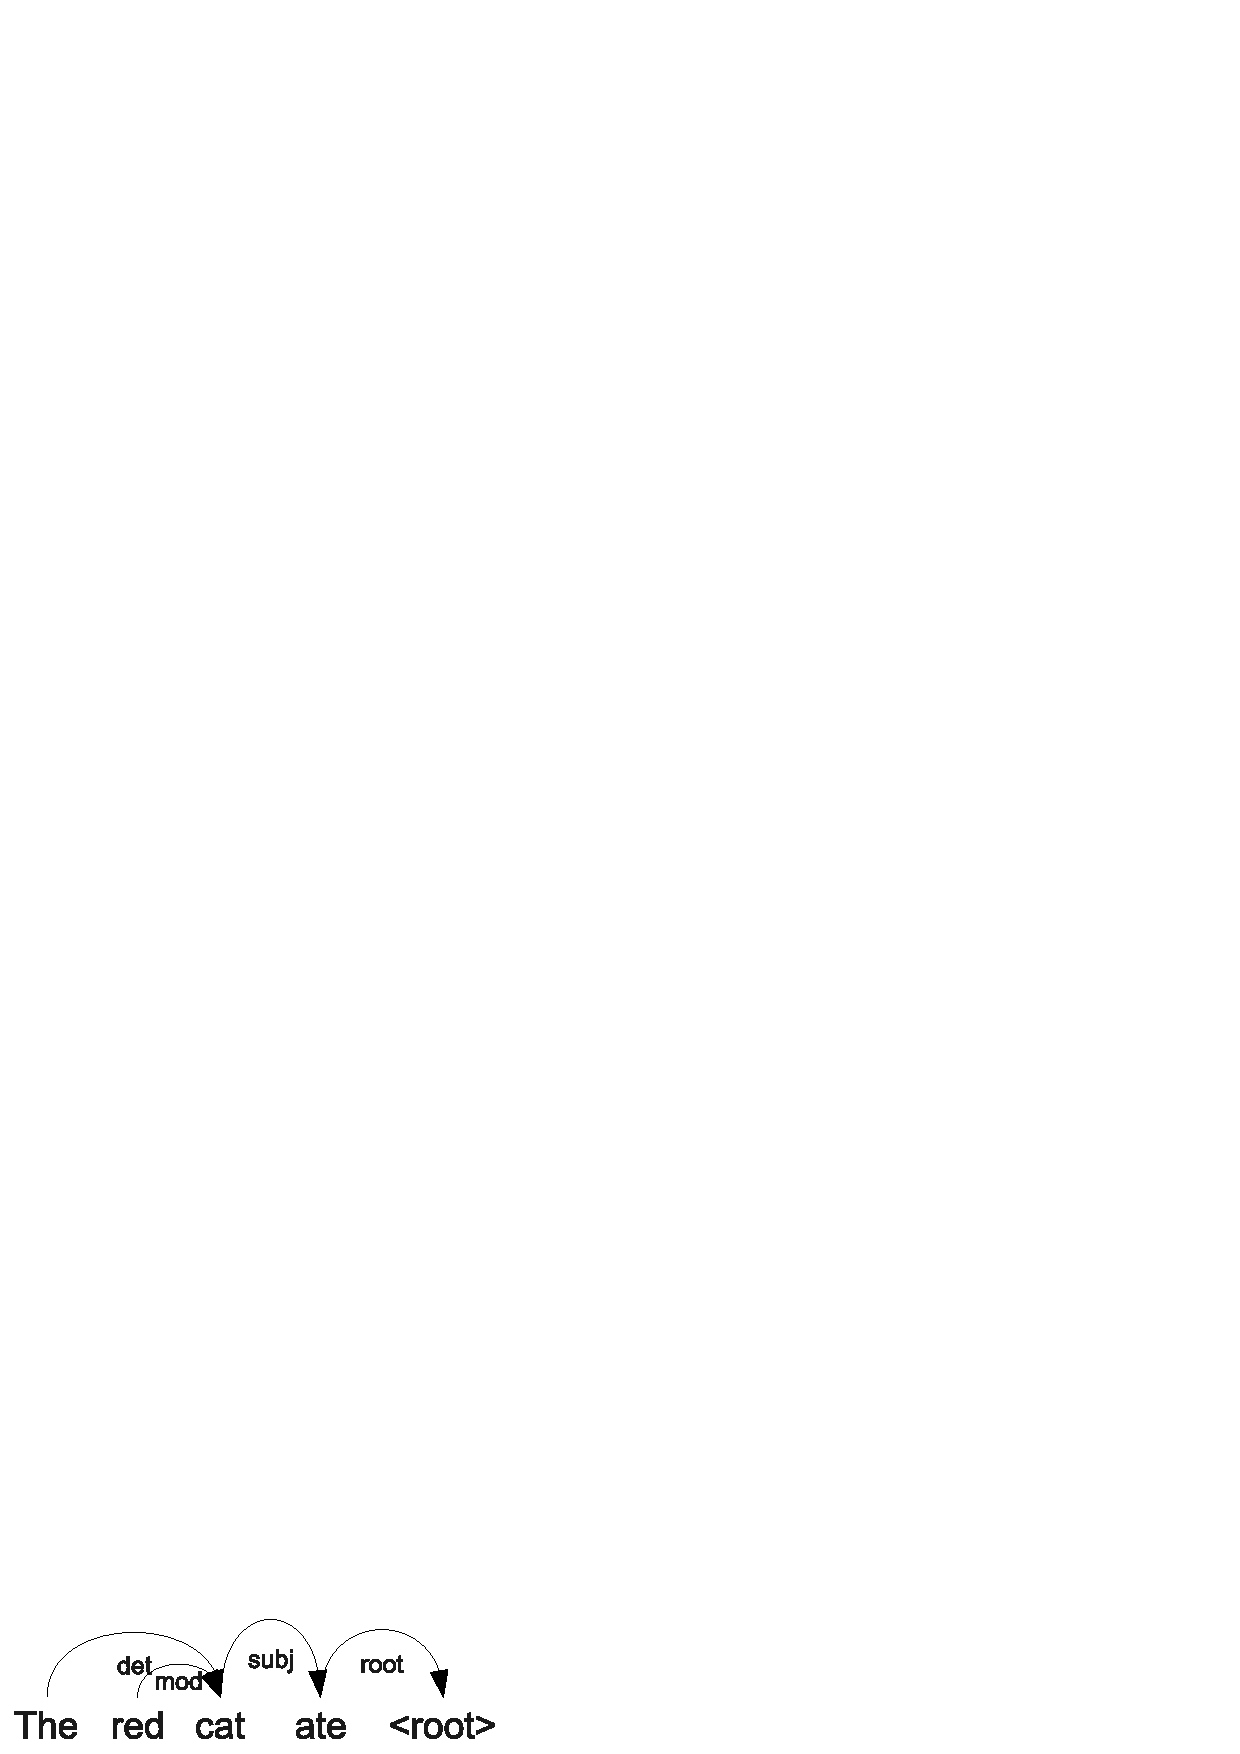
\includegraphics[scale=0.6]{dpm-example-ref.png} & 
    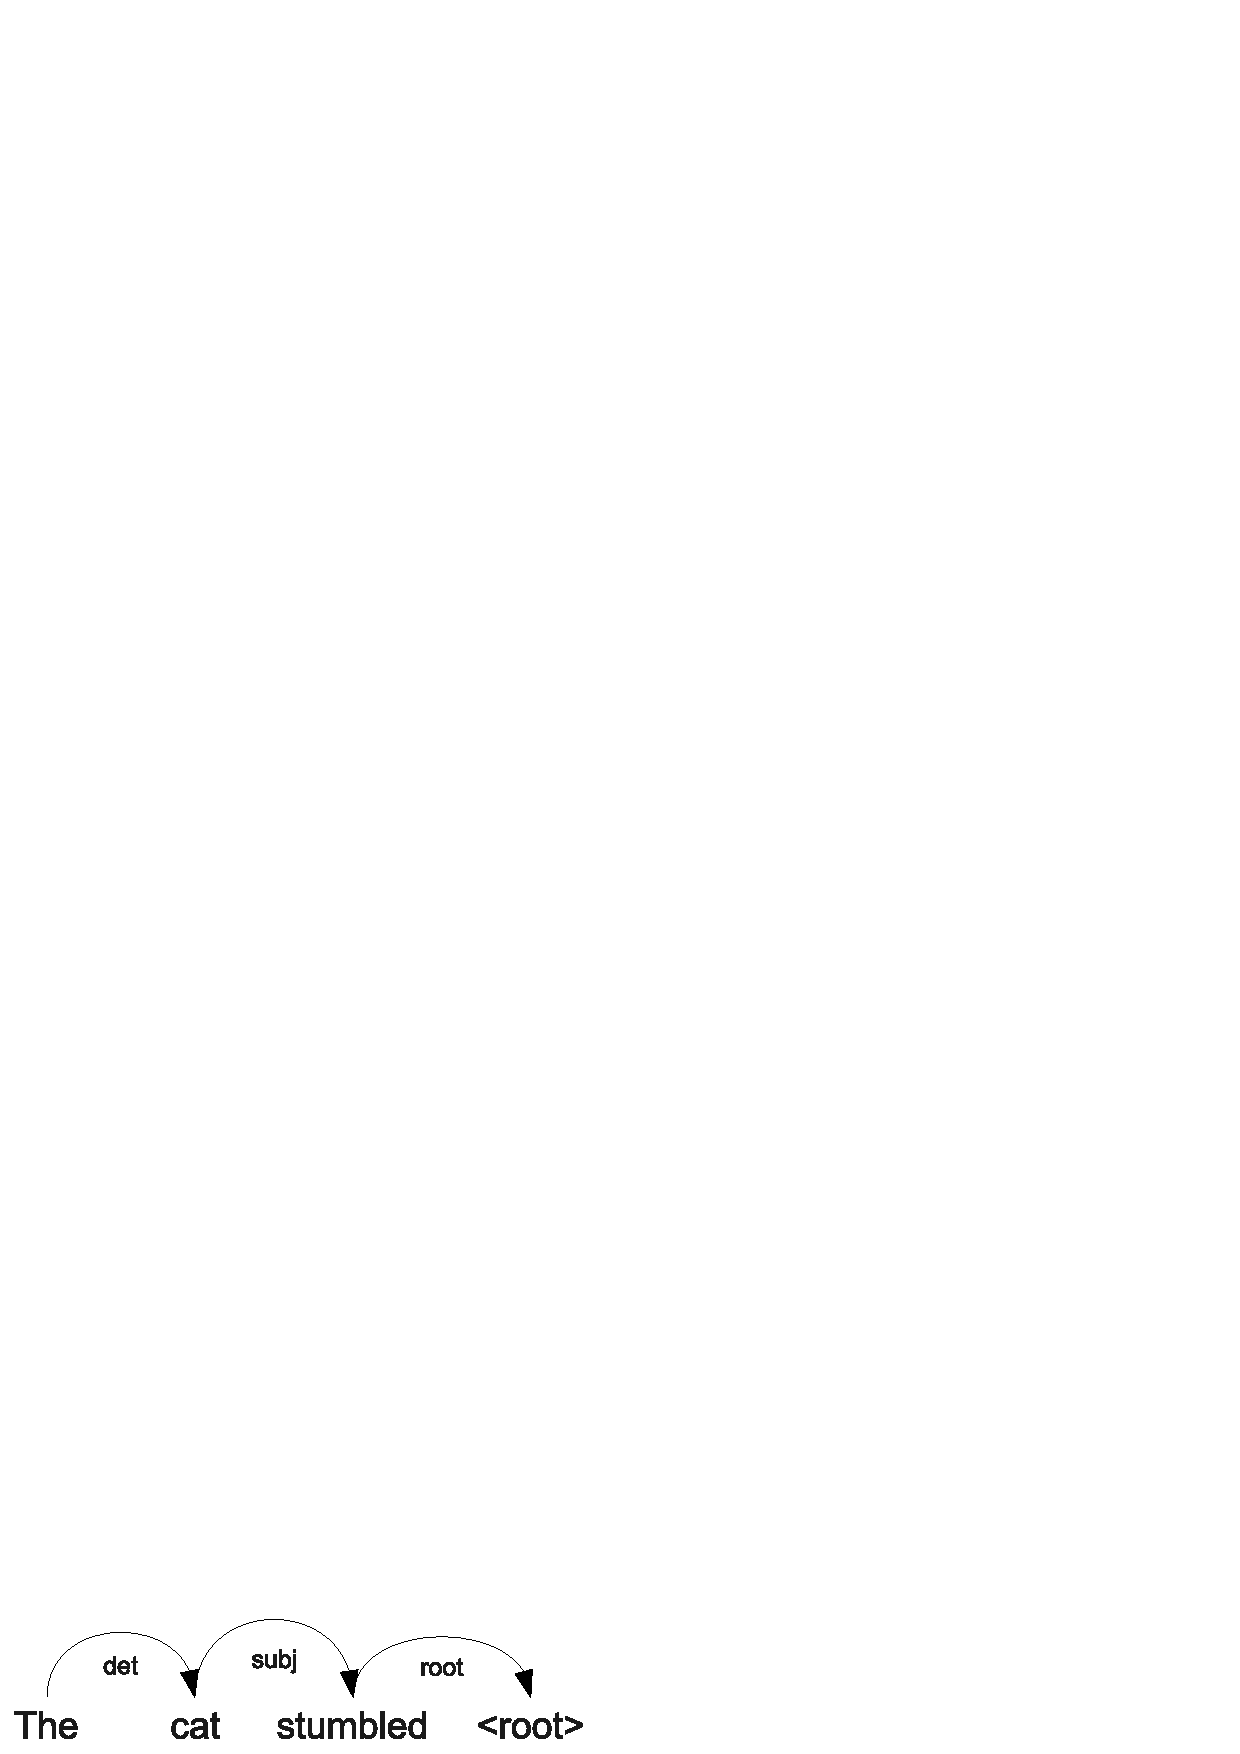
\includegraphics[scale=0.6]{dpm-example-hyp.png}\\
    \textbf{$dlh$ list} &
    \begin{tabular}{@{$\langle$}c@{,~}c@{,~}c@{$\rangle$}}
      the & \arclabel{\texttt{det}}  &  cat \\
      red & \arclabel{\texttt{mod}}  &  cat \\
      cat & \arclabel{\texttt{subj}} &  ate \\
      ate & \arclabel{\texttt{root}} &  $<$root$>$ \\
    \end{tabular} & 
    \begin{tabular}{@{$\langle$}c@{,~}c@{,~}c@{$\rangle$}}
      the &      \arclabel{\texttt{det}}  &  cat \\
      cat &      \arclabel{\texttt{subj}} &  stumbled \\
      stumbled & \arclabel{\texttt{root}} &  $<$root$>$ \\
    \end{tabular}\\
  \end{tabular}\\
  Precision$_{dlh}$ is $\frac{1}{3}$ and Recall$_{dlh}$ is
  $\frac{1}{4}$, yielding  $\DPM{dlh} = F = \frac{2}{7} = 0.286$
  \caption{Example hypothesis and reference dependency trees and the $dlh$ decomposition of each.}
  \label{fig:dpmexample}
\end{figure*}
Figure~\ref{fig:dpmexample} demonstrates a toy example of the
bags-of-dependencies extracted from a hypothesis and reference
tree.  In the examples presented here, we extract only $dlh$
dependencies, which are tuples of the form $\langle \textrm{Dependent},
\textrm{arc-Label}, \textrm{Head} \rangle$.
We describe different variants in this family below, and compare their
effectiveness in section~\ref{sec:facorr}.

\subsection{\DPMempty{} variations in subtree extraction}
Different members of the \DPMempty{} family may extract different
subtrees.  In this section, we denote the set of tree-components extracted via a
trailing subscript: \DPM{dlh} extracts all $\langle
\textrm{Dependent}, \textrm{arc-Label}, \textrm{Head} \rangle$ subtree
tuples for the $F$ measure, which is equivalent (modulo the
dependency-extraction methods) to labeled \textsc{SParseval} and the
\newcite{owczarzak07labelleddepseval} \textbf{d} measure.
\DPM{dl,lh}, by contrast, extracts all the subtrees $\langle
\textrm{Dependent}, \textrm{arc-Label} \rangle$ and $\langle
\textrm{arc-Label}, \textrm{Head} \rangle$, which is equivalent to the
\newcite{owczarzak07labelleddepseval} \textbf{d\_var} method (again,
modulo the dependency-extraction method).  In the example trees in
figure~\ref{fig:dpmexample}, the hypothesis tree produces the following
six items for scoring with \DPM{dl,lh}:
\begin{center}
  \begin{tabular}{cc}
    $dl$ & $lh$ \\
    \hline
    \begin{tabular}{@{$\langle$}c@{,~}c@{$\rangle$}}
      the & \arclabel{\texttt{det}}  \\
      cat & \arclabel{\texttt{subj}} \\
      stumbled & \arclabel{\texttt{root}} \\
    \end{tabular} &
    \begin{tabular}{@{$\langle$}c@{,~}c@{$\rangle$}}
      \arclabel{\texttt{det} } &  cat \\
      \arclabel{\texttt{subj}} &  stumbled \\
      \arclabel{\texttt{root}} &  $<$root$>$ \\
    \end{tabular}\\
  \end{tabular}
\end{center}
so that Precision$_{dl,lh}$ is $\frac{3}{6}$ and Recall$_{dl,lh}$ is
$\frac{3}{8}$, giving a \DPM{dl,lh} of $\frac{3}{7} = 0.429$ for the
example.

\subsection{\DPMempty{} variations in binning subscores}
When the \DPMempty{} measure is composed of more than one class of
tuple (e.g.\ \DPM{dl,lh}, but not \DPM{dlh}), we may consider adopting
a strategy like BLEU \cite{papineni02bleu} or the syntactic measures
from \newcite{liu05syntaxformteval} and compute an average of
subscores over each tuple class. We define a binned DPM \bDPM{} as the
harmonic mean of separate precision and recall
scores\footnote{\bDPM{} differs from both \newcite{papineni02bleu}
  and \newcite{liu05syntaxformteval} in that the earlier metrics use
  averages over precision subscores, necessitating an ``anti-gaming''
  brevity penalty (in BLEU), while the \bDPM{} measure is an average
  across precisions and recalls.} for each class of tuple involved,
rather than simple $F$ (the harmonic mean of a single precision and
recall score over all the tuples together).

\subsection{\DPMempty{} variations using $n$-best lists and expected counts}
%% Multiple parses
Since the dependency structure is hidden, we may also be interested in
exploring alternative dependency structures (in both hypothesis and
reference) predicted by the parser, to cope with both error in the
parser and ambiguity in the translation hypothesis and
reference. \DPMempty{} is well-defined over the $n$-best list of
dependency-structures: when $n>1$, \DPMempty{} uses the expectation of
bags-of-subtrees (rather than the bags-of-subtrees derived from the
1-best parse).

An expectation requires a probability distribution over the $n$-best
list, and we consider three options: uniform, the parser
probabilities, and a flattened version of the parser probabilities
such that $\tilde{p}(x) = \frac{p(x)^\gamma}{\sum_ip(i)^\gamma}$
(where $\gamma$ is a free parameter) to account for the fact that the
parser tends to be over-confident.  In all cases, the probabilities
are normalized to sum to one over the the $n$-best list, where the
maximum $n$ in this work is 50.  The uniform distribution ($\gamma =
0$) is intended to be equivalent to the
\newcite{owczarzak07labelleddepseval} \textbf{d\_50} and
\textbf{d\_50\_var} measures.\footnote{Since
  \newcite{owczarzak07labelleddepseval} report no use of parse
  weights, \textbf{d\_50} and \textbf{d\_50\_var} may be using a sum
  of counts over the 50-best list rather than expected-counts over a
  uniform distribution. These two approaches are equivalent --- so
  long as the $n$-best list is always the same length for hypothesis
  and reference.  In our implementation
  (section~\ref{sec:implementation}), the $n$-best list does not
  always reach 50 candidate parses on short sentences, so the
  expectation matches our intent better than a sum of counts over the
  $n$-best.}
%
We note in
table~\ref{tab:measurecorrespondences} those measures in the
\DPMempty{} family that correspond to
\newcite{owczarzak07labelleddepseval} measures.
\begin{table}
  \centering
  \begin{tabular}{|r|r|r||l|}
    \hline
    \multicolumn{3}{|c||}{\DPM{}} & \newcite{owczarzak07labelleddepseval}\\
    Sub-graph & $n$ & $\gamma$ & \\ % & \textbf{d\_*} measure \\
    \hline
    $dlh$ & 1  & --- & \textbf{d} \\
    $dlh$ & 50 & 0   & \textbf{d\_50} \\
    \hline
    $dl,lh$ & 1 & --- & \textbf{d\_var} \\
    $dl,lh$ & 50 & 0 & \textbf{d\_50\_var}\\
    \hline
  \end{tabular}
  \caption{\textbf{Correspondences between the \DPMempty{} family of
      measures and \newcite{owczarzak07labelleddepseval} \textbf{d\_*} measures.}
    Differences between dependency extraction methods are ignored for
    these equivalencies.}
  \label{tab:measurecorrespondences}
\end{table}
% TO DO: MO note: if tight on space, delete this table.

\subsection{Implementation of the \DPMempty{} family}
\label{sec:implementation}
In principle, the \DPM{} family of measures may be implemented with
any parser that generates a dependency graph (a single labelled arc
for each word, pointing to its head-word). Prior work
\cite{owczarzak07labelleddepseval} on related
measures has used an LFG parser \cite{cahill04lfg} or
an unlabelled dependency tree \cite{liu05syntaxformteval}. 

%
In this work, we use a state-of-the-art PCFG (the first stage of
\newcite{charniak-johnson:2005:ACL}) and context-free head-finding
rules \cite{magerman95headfinding} to generate a 50-best list of
dependency trees for each hypothesis and reference translation.  We
use the parser's default Wall Street Journal training parameters.
Head-finding uses the Charniak parser's rules, with three
modifications: prepositional and complementizer phrases choose nominal
and verbal heads respectively (rather than functional heads) and
auxiliary verbs are modifiers of main verbs (rather than the
converse).

Having constructed the dependency tree, we label the arcs as $d
\stackrel{A/B}{\to} h$, where the arc label $A/B$ between dependent
$d$ and its head $h$ is composed of $A$ (the lowest constituent-label
headed by $h$ and dominating $d$) and $B$ (the highest constituent
label headed by $d$). 
\begin{figure}
  % \centering
  \Tree
  [.\headlabel{S}{stumbled}
    [.\headlabel{NP}{cat}
      [.\headlabel{DT}{the} the ]
      [.\headlabel{NN}{cat} cat ]
    ]
    [.\headlabel{VP}{stumbled} 
      [.\headlabel{VBD}{stumbled} stumbled ]
    ]
  ]
  \\
  \begin{center}
    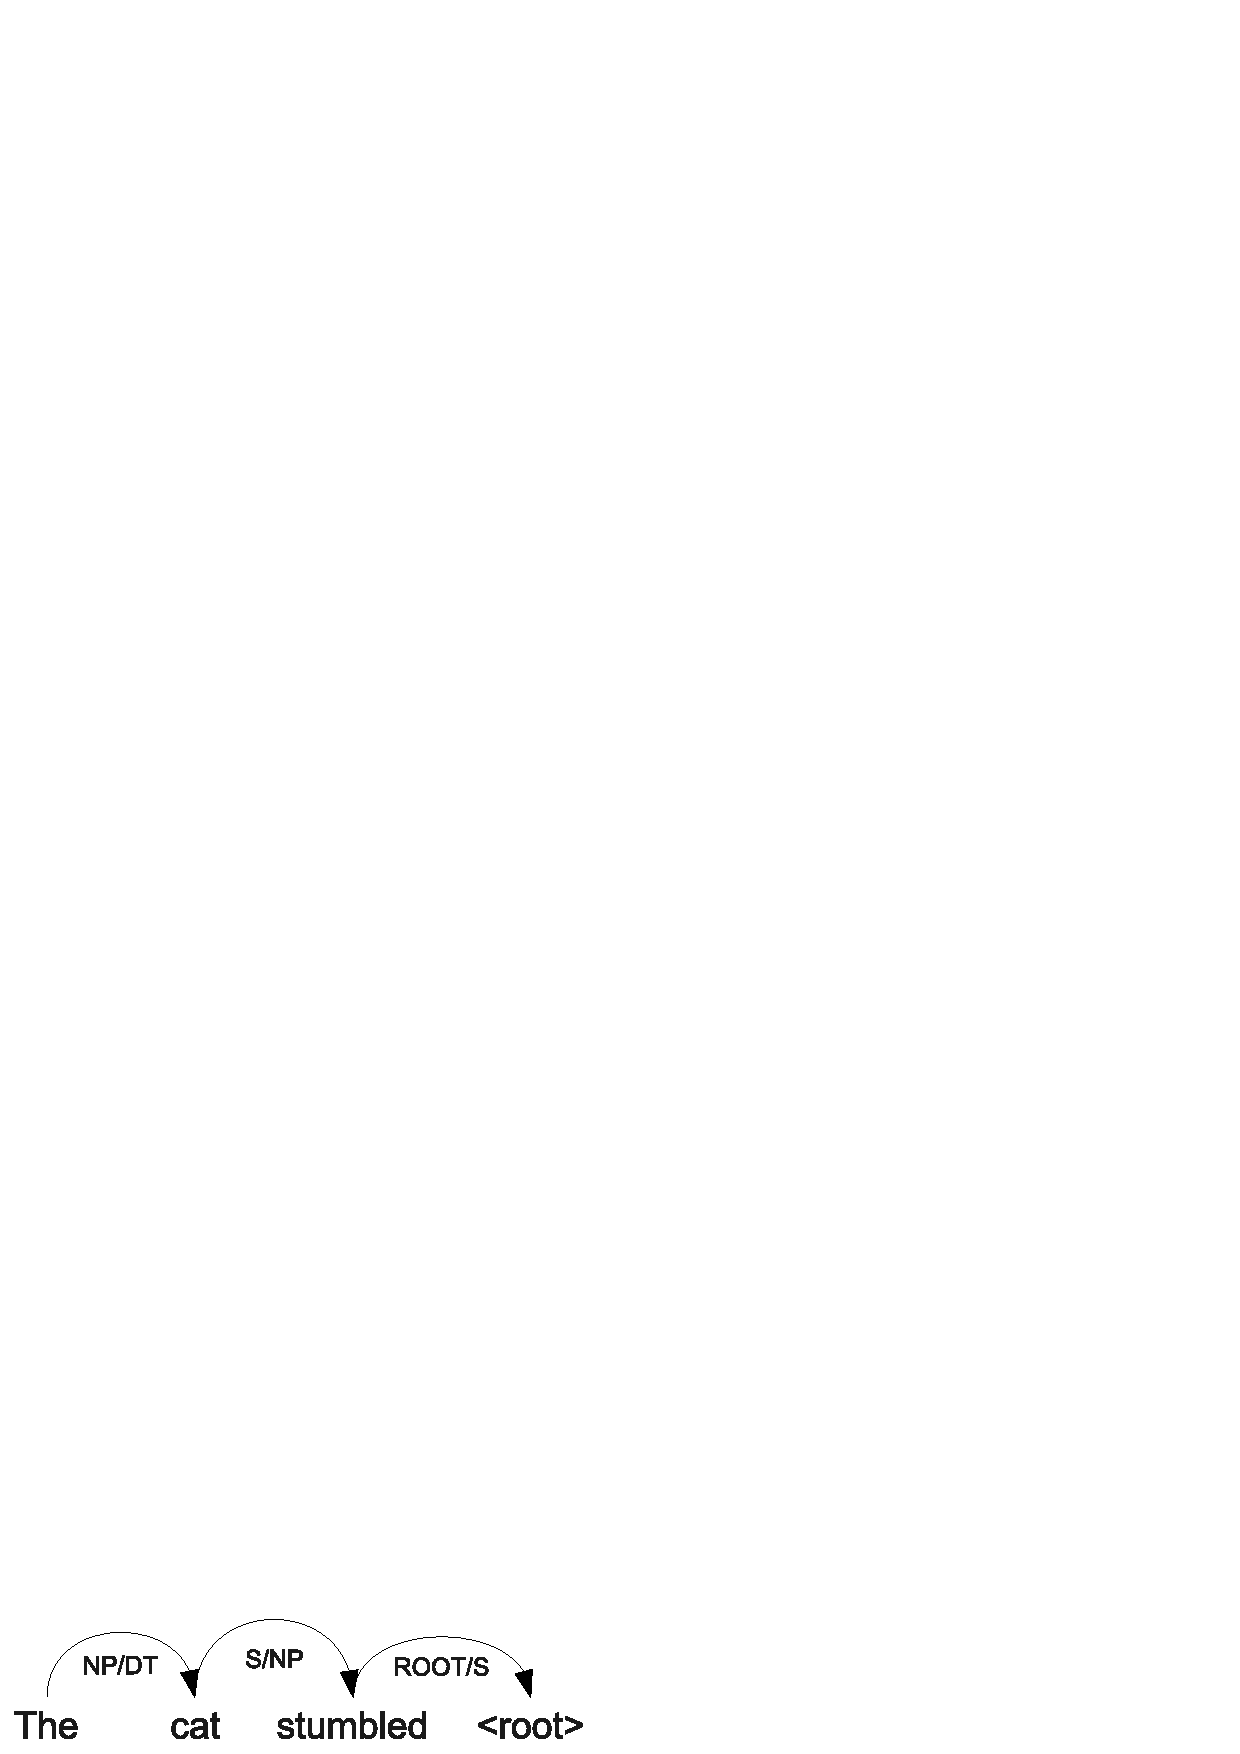
\includegraphics[scale=0.6]{dpm-example-depextract.png}
  \end{center}
  \caption{An example constituent tree (heads of each constituent are
    listed small below the label) and the labelled dependency tree
    derived from it using the strategy described in
    section~\ref{sec:implementation}.}
  \label{fig:depextract}
\end{figure}
For example, in figure~\ref{fig:depextract}, the S node is the
lowest node headed by \emph{stumbled} that dominates \emph{cat}, and
the NP node is the highest constituent label headed by \emph{cat}, so
the arc between \emph{cat} and \emph{stumbled} is labelled \arclabel{S/NP}.
%
This strategy is very similar to one adopted in the reference
implementation of labelled-dependency \textsc{SParseval}, and may be
considered as an approximation of the rich semantics generated by
\cite{cahill04lfg} or another heavily knowledge-engineered
parser, but with much less knowledge-engineering required.

The $A/B$ labels are not as descriptive as the LFG semantics, but they
have a similar resolution, e.g.\ the $\stackrel{S/NP}{\to}$ arc label
usually represents a subject dependent of a sentential verb.

\section{Correlation with human judgments of fluency \& adequacy}
\label{sec:facorr}

To select a good member of the \DPMempty{} family, we explore the
correlation of these measures against a corpus of human judgments of
fluency and adequacy. 

\subsection{Corpus}

For these experiments, we use LDC Multiple Translation Chinese corpus
parts 2~\cite{LDC03MTC2} and 4~\cite{LDC06MTC4}.  These corpora
include multiple human judgments of fluency and adequacy for each
sentence, with each judgment using a different human judge and a
different reference translation.  For a rough\footnote{Our segment
  count differs from \newcite{owczarzak07labelleddepseval}, who report
  16,800 segments over the same corpus. We find baseline correlations
  (BLEU$_4$ and TER) lower than those reported there as well, so the
  results presented here are not directly comparable with that paper,
  though we demonstrate similar gains over those baselines in
  essentially the same corpus (section~\ref{sec:facorr:newdeps}).}
comparison with \newcite{owczarzak07labelleddepseval}, we treat each
judgment as a separate segment.
%
This treatment of this corpus yields 16,815 tuples of
$\langle$hypothesis, reference, fluency, adequacy$\rangle$.  In these
experiments, we extend this tuple with automatic scores derived from
$\langle$hypothesis, reference$\rangle$ and examine the
correlations\footnote{The independence of each of these segments is
  questionable, since the same hypothesis translations are used in
  multiple items, but for the sake of methodological comparison with
  prior work, this strategy is preserved.}  between those automatic
scores and the arithmetic mean of the fluency and adequacy measures.
% TO DO: anything more to say here. 

\subsection{Utility of alternative dependency extraction}
\label{sec:facorr:newdeps}
Our research suggests that the dependency extraction strategy from
section~\ref{sec:implementation} works in place of the richer
semantics from an LFG parser.  
\begin{table}
  \centering
  \begin{tabular}{r|d}
    \textbf{Measure} & \multicolumn{1}{c}{$r$} \\
    % vs.\ $\frac{\mathrm{fl} + \mathrm{ad}}{2}$} \\
    \hline
    \DPM{dl,lh} ($\sim$\textbf{d\_var}) & 0.226\\
    \DPM{dlh} ($\sim$\textbf{d}) & 0.185 \\
    TER & -0.173 \\
    BLEU$_4$ & 0.139 \\
  \end{tabular}
  \caption{
    Correlation of various measures with the average of fluency and
    adequacy over the sentences in the MTC corpus. These \DPMempty{} results use
    only the one-best parse ($n=1$).
    \label{tab:facorr:statsparser}}
\end{table}
The results in table~\ref{tab:facorr:statsparser}, which use only the
top parse for each sentence, are very similar to those reported in
\newcite{owczarzak07labelleddepseval}, in that the syntactic measure
\DPM{dl,lh} ($\sim$\textbf{d\_var}) is much-better correlated with
human judgment than the non-syntactic measures BLEU$_4$ and TER.
%% TO DO: look at the following thought
% The difference between the syntactic and non-syntactic measures are
% here not quite as large as the differences reported in earlier work,

\subsection{Alternative dependency sub-graphs}

The \DPMempty{} family allows us to easily explore alternative
sub-graphs of the dependency graph, and we find that we achieve small
improvements in correlation with human judgments by including the
unigram ($1g$) and bigram ($2g$) in the dependency-tree decomposition,
ignoring the dependency arc.  \newcite{owczarzak07labelleddepseval}
found that their original proposal, \textbf{d}, scoring full
dependent-arc-head triples, was not as well-correlated with human
judgment as \textbf{d\_var}, which examined only dependent-arc and
arc-head tuples. Table~\ref{tab:facorr:statsparser} confirms this as
well for a statistical constituent parser with simple
dependency-extraction.  In table~\ref{tab:facorr:subgraphs}, we extend
this search to consider whether it is useful to include other
subgraphs of the dependency tree into the bag of tree-fragments to be
scored.
\begin{table}
  \centering
  \begin{tabular}{r|d}
    \textbf{Measure} & \multicolumn{1}{c}{$r$}\\
    % vs.\ $\frac{\mathrm{fl} + \mathrm{ad}}{2}$} \\
    \hline
    \DPM{1g,2g,dl,lh} & 0.237\\
    \DPM{1g,dl,lh}   & 0.234\\
    \\
    \DPM{1g,2g}($\equiv\BoNG{2}$)     & 0.227 \\
    \DPM{dl,lh}     & 0.226\\
    \\
    % \DPM{d} ($\equiv$ bag-of-words F) & 0.214 \\
    \DPM{1g,dl,dlh} & 0.227\\
    \DPM{dlh} & 0.185 \\
    TER       & -0.173 \\
    BLEU$_4$  & 0.139 \\
  \end{tabular}
  \caption{
    As in table~\ref{tab:facorr:statsparser}, but with 
    alternative dependency-graph constituents to compute the $F$
    measure.  Again, $n=1$ for all \DPMempty{} correlations.
    \label{tab:facorr:subgraphs}}
\end{table}

Table~\ref{tab:facorr:subgraphs} shows that we can combine the
benefits of string-local $n$-grams (\DPM{1g,2g}) with the benefits of
dependency information (\DPM{dl,lh}) for a further improved
correlation with human judgment, with the best correlation in
\DPM{1g,2g,dl,lh}. Including progressively larger chunks of the
dependency graph (as in \DPM{1g,dl,dlh}, which is inspired by the
BLEU$_k$ idea of progressively larger $n$-grams) does not seem to be
an improvement over \DPM{dl,lh}.

\subsection{Binning subscores with \bDPM{}}
BLEU \cite{papineni02bleu} and the related NIST
\cite{doddington02nist} measure, as well as the earlier proposed
syntactic measures \cite{liu05syntaxformteval}, choose to sort their
components into bins on length, and take average scores over those
bins.  \newcite{owczarzak07labelleddepseval} measures, by contrast, and
the \DPM{} measures by extension, score all components together in one
bin, measuring precision and recall of all bins combined.
\begin{table}
  \centering
  \begin{tabular}{r|d}
    \textbf{\DPM{} measures} & \multicolumn{1}{c}{$r$} \\
    % vs.\  $\frac{\mathrm{fl} + \mathrm{ad}}{2}$} \\
    \hline
    \DPM{1g,2g,dl,lh}  & 0.237\\
    \bDPM{1g,2g,dl,lh} & 0.217 \\
%     \\
    \DPM{1g,dl,lh}  & 0.227\\
    \bDPM{1g,dl,lh} & 0.212 \\
    \DPM{dl,lh} & 0.226\\
    \bDPM{dl,lh} & 0.208 \\
%     \hline
%     \DPM{d} & 0.214 \\
    \hline
    \hline
    \textbf{$n$-gram measures} \\
    \hline
    \BoNG{2} & 0.227 \\
    \bBoNG{2} & 0.215\\
    BLEU$_2$ & 0.211 \\
    \hline
    \BoNG{3} & 0.227 \\
    BLEU$_3$ & 0.179 \\
    \bBoNG{3} & 0.177\\
    \hline
    \BoNG{4} & 0.225 \\
    BLEU$_4$ & 0.139 \\
    \bBoNG{4} & 0.135 \\
    \hline
%     TER & -0.173 \\
  \end{tabular}
  \caption{
    As in
    table~\ref{tab:facorr:subgraphs}, but also exploring the
    possibility of binning syntactic and $n$-gram components of
    different sizes into  subscores and combining, on the model of
    BLEU.  $n=1$ for all \DPM{} measures.
    \label{tab:facorr:multibin}
  }
\end{table}  
In table~\ref{tab:facorr:multibin} we explore which strategy is
preferred, and show that binning with \bDPM{} does not improve
correlations for the syntactic measures.  In fact, \bDPM{} measures
are consistently worse-correlated than their corresponding \DPMempty{}
measure.

For comparison, we try the same approach with $n$-grams, comparing
\bBoNG{k} (the
harmonic mean of $k$ precisions and $k$ recalls) to \BoNG{k} (a
single $F$ over one bin of $n$-grams of lengths 1-$k$), and
we find that the single bin again performs better than the separated
bins.  For comparison, the \BoNG{1} (a bag-of-words $F$) has an $r$ of
0.214 over the same corpus; thus, for $n$-grams, the main improvement
is in moving from 1-grams to 2-grams, but only for the non-binned
variants.  We also include BLEU in table~\ref{tab:facorr:multibin},
which allows a comparison of BLEU's strategy (average precision and
brevity penalty) to an $F$-style harmonic mean of precision and recall
(binned separately and together).  We find that BLEU$_k$ does about as
well as the corresponding \bBoNG{k}, while the \BoNG{k} does
consistently better than BLEU$_k$, especially for larger $k$.
% TO DO: Worth noting that \bDPM{dl,lh} is actually worse than \DPM{d}?

% note: \DPM{d,dh} actually performs \emph{worse} (0.224) than
%   \BoNG{2} (0.227).  Looking at alternative parses doesn't help really
%   at all, either.  Both of these suggest that arc labels --- even more
%   than arc-positions --- make a difference here.   Is this
%   worth discussing? Exploring POS-tagging matches?

\subsection{Using parse $n$-best lists}
We explore the use of multiple parses in
table~\ref{tab:facorr:multiparse}, which presents \DPM{} variants with
$\gamma=0$ of the most successful \DPM{} sub-graph lists shown in previous
tables.
\begin{table}
  \centering
  \begin{tabular}{r|r|d}
    \textbf{Measure} & \textbf{parameters} & \multicolumn{1}{c}{$r$}\\
    % vs.\ $\frac{\mathrm{fl} + \mathrm{ad}}{2}$} \\
    \hline
    \DPM{1g,2g,dl,lh} & $\gamma=0, n={50}$ & 0.239 \\
    \DPM{1g,2g,dl,lh} &  $n=1$ & 0.237\\
    \DPM{1g,dl,lh} & $\gamma=0, n={50}$ & 0.237 \\
    \DPM{1g,dl,lh} &  $n=1$ & 0.234\\
%    \\
    \DPM{dl,lh} ($\sim\textbf{d\_50\_var}$) & $\gamma=0, n={50}$  & 0.234 \\
    \DPM{dl,lh} ($\sim\textbf{d\_var}$)& $n=1$ & 0.226\\
  \end{tabular}
  \caption{
    As in table~\ref{tab:facorr:subgraphs}, but considering variants
    of the best \DPM{} measures uniform probability distribution over
    multiple parses ($\gamma=0, n=50$).
    \label{tab:facorr:multiparse}}
\end{table}
We use $\gamma=0$ (uniform probability over the $n$-best list) to
compare as closely as possible to
\newcite{owczarzak07labelleddepseval}, which uses a parser with ranks
but no weights.

We find that using multiple parses with a uniform distribution
improves correlations further, although the improvement from varying
the dependency-tree sub-graphs is not as large for $n=50$ variants of
\DPM{} as for $n=1$ variants.
% \footnote{Although the \BoNG{3} correlations are
%   impressive, they cannot take advantage of the extra knowledge source
%   provided by the parser, since they only use surface features.}

%% Not sure how true this next thought is:
% Also note that the improvements are not as large
%   with this implementation as the improvements reported in
%   \cite{owczarzak07labelleddepseval}.  \footnote{possible that the
%     alternative LFG dependencies are more semantially-diverse/less
%     subject to (e.g.) morphological scatter, so $n$-best is more
%     diverse in LFG?  a note for future work?}

\subsection{Including parse confidence}
Since the parser in our implementation provides a confidence in each
parse, we explore the use of that confidence with the $\gamma$ free
parameter.
\begin{table}
  \centering
  \begin{tabular}{r|l||d}
    \multicolumn{3}{c}{\DPM{1g,2g,dl,lh}}  \\
    \multicolumn{1}{c|}{$n$} & \multicolumn{1}{c||}{$\gamma$} & \multicolumn{1}{c}{$r$} \\
    \hline
    % vs.\ $\frac{\mathrm{fl} + \mathrm{ad}}{2}$} \\
    \hline
    % TO DO: fill these in.
    50 & {0.25} & 0.240 \\
    50 & {0.5\phantom{0}}  & 0.240 \\
    50 & {0.75} & 0.240 \\
    50 & {1}    & 0.239 \\
    50 & 0      & 0.239 \\
     1 & ---    & 0.237 \\
    \hline
  \end{tabular}~
  \begin{tabular}{r|l||d}
    \multicolumn{3}{c}{\DPM{dl,lh}}   \\
    \multicolumn{1}{c|}{$n$} & \multicolumn{1}{c||}{$\gamma$} & \multicolumn{1}{c}{$r$} \\
    \hline
    % \end{tabular}\\
    % \begin{tabular}{r|d}
    %   \textbf{Measure} & \multicolumn{1}{c}{$r$ vs.\
    %     $\frac{\mathrm{fl} + \mathrm{ad}}{2}$} \\
    \hline
    50 & {0.25} & 0.234 \\
    50 & {0.5} & 0.234 \\
    50 & 0 & 0.234 \\
    50 & 0.75 & 0.233 \\
    50 & {1} & 0.232 \\
    1 & --- & 0.226 \\
    \hline
%     \hline
%     \textbf{Comparison measures}\\
%     \hline
%     (\BoNG{3}) & (0.227) \\
%     (\BoNG{2}) & (0.227) \\
%     (TER) & (-0.173) \\
%     (BLEU$_4$) & (0.139) \\
  \end{tabular}
  \caption{
    As in table~\ref{tab:facorr:multiparse}, but
    considering various values of $\gamma$ and $n$ for two different
    \DPMempty{} sub-graph lists ($dl,lh$ and $1g,2g,dl,lh$).
%   All variants of EDPM use
%     the 50-best parses.
    \label{tab:facorr:parseweight}}
\end{table}
Table~\ref{tab:facorr:parseweight} explores various ``flattenings''
(values of $\gamma$) of the parse confidence in the \DPM{}
measure. $\gamma=1$ is not always the best, suggesting that the parse
probabilities $p(\mathrm{tree}|\mathrm{words})$ are overconfident. We
find that $\gamma=0.25$ is generally the best flattening of the parse
confidence for the variants of \DPM{} that we have tested.  The
differences are small, but the trends are consistent across the
variants.

\subsection{Summary}

In this section, we have presented experiments exploring a number of
parameters to the \DPMempty{} measure. The experiments suggest a
best-case variant \myEDPM{}, where we set:
\begin{displaymath}
  \myEDPM{} = \DPM{1g,2g,dl,lh}, n=50, \gamma=0.25
\end{displaymath}
in which we choose a $1g,2g,dl,lh$ sub-graph decomposition based on
the improvements from better sub-graphs
(table~\ref{tab:facorr:subgraphs}), multiple parses ($n=50$) based on
table~\ref{tab:facorr:multiparse}, and $\gamma=0.25$, hinted at by
table~\ref{tab:facorr:parseweight}.  We use these \myEDPM{}
parameter-settings in the experiments exploring correlations with HTER
(below).


% TO DO: MO says: I really don't like the final result tied to a
% specific gamma.  the best gamma is a parameter that would be tuned
% for particular tasks and parsers in the same what that one might
% tune n for n-best, and you don't have 50 in the name. 

% MO: You could avoid the hat by not using EDPM until this section.
% JGK: TO DO: don't use EDPM until here.

\section{Correlations with HTER}
\label{sec:hter}

Having chosen \myEDPM{} as a good candidate member of the \DPMempty{}
family, we explore its utility on another task: predicting the
human-targeted translation edit rate (HTER) on the (unsequestered) GALE 2.5
% \cite{olive06gale}
evaluation results.

\subsection{Corpus}

The GALE 2.5 translation corpus is made up of system translations into
English from three sites.
% MO added:
The three sites all use system combination to integrate results from
multiple systems, some of which are phrase-based and some which may
use syntax on either the source or target side. No system provided
system-generated parses.
%
The corpus being translated comes from
Arabic and Chinese in four genres: \texttt{bc} (broadcast
conversation), \texttt{bn} (broadcast news), \texttt{nw} (newswire),
and \texttt{wb} (web text), with corpus sizes shown in
table~\ref{tab:galestats}.
\begin{table}
  \centering
  \begin{tabular}{r|rr|rr|rr}
     & \multicolumn{2}{c|}{Arabic} & \multicolumn{2}{c|}{Chinese}
     & \multicolumn{2}{c}{Total}\\
     & doc & sent & doc & sent & doc   & sent\\
     \hline
     \texttt{bc}    & 59  & 750 & 56 & 1061 & 115 & 1811\\
     \texttt{bn}    & 63  & 666 & 63 & 620  & 126 & 1286\\
     \texttt{nw}    & 68  & 494 & 70 & 440  & 138 & 934 \\
     \texttt{wb}    & 69  & 683 & 68 & 588  & 137 & 1271\\
     \hline
     Total & 259 & 2593& 257& 2709 & 516 & 5302\\
  \end{tabular}
  \caption{Corpus statistics for the GALE 2.5 translation
    corpus.}
  \label{tab:galestats}
\end{table}
The corpus includes one English reference translation $r_i$
\cite{gale08phase2_5references} for each sentence $i$ and a system
translation $t_{i,z}$ for each of the three systems
$z$. Additionally, each of the system translations of each segment $i$
has a corresponding human-targeted reference aligned at the sentence
level, so we have available the HTER score of each segment
$s_{\textsc{hter}}(t_{i,z})$ at both the sentence and document level.

\subsection{Prediction of $\Delta$HTER per-document}

We evaluate our new measure \myEDPM{} by testing its prediction of
improvements in HTER over different translations of a document.
We name one of the three translation systems arbitrarily as baseline
$b$ and define
\begin{eqnarray}
  \label{eq:delta}
  \Delta s(i,b,z) & = & s(t_{i,z}) - s(t_{i,b})
\end{eqnarray}
as a measure of change % in measure $s$
that system $z$ provides over segment $i$ with respect to system $b$
(by providing translation $t_{i,z}$ instead of $t_{i,b}$).
% $\Delta_b(s,t_{i,z})$ may be either positive or negative.

We would like an automatic measure $s$ that provides a good
correlation $r$ between $\Delta s$ and $\Delta \textsc{hter}$.  For
each of the 516 documents\footnote{Using per-document comparison
  avoids the problems of per-sentence comparisons, e.g.\ that BLEU
  falls to zero too easily on a sentence.} in the corpus described in
table~\ref{tab:galestats}, for each of the three pairs of systems, we
generate the $\Delta s$ scores, ordering the systems such that
$\Delta\textsc{hter} \geq 0$ for each document pair.

% For candidate score
% measures $s$ (including target measure \textsc{hter}), we generate
% three $\Delta s$ data (all possible system pairs, ordered such that
% $\Delta$\textsc{hter} is always positive) for
% % Using this $\Delta_b$ measure for each score, we have two data for
% each document of the 516 documents in the corpus
% described in table~\ref{tab:galestats}.

Table~\ref{tab:hter:perdoc1} shows the per-document correlations with
$\Delta\textsc{hter}$ over this set of data, broken out into per-genre
and per-language correlations.

\begin{table}
  \centering
  \begin{tabular}{r|r|r||r}
     \multicolumn{1}{c|}{Measure $s$} 
     & \multicolumn{1}{c|}{all-Arabic} &
     \multicolumn{1}{c||}{all-Chinese} &\multicolumn{1}{c}{all}\\
    \hline{}
    TER      &  0.51 &  0.19 &  0.39 \\
    BLEU$_4$ & -0.40 & -0.19 & -0.32 \\
    \myEDPM  & 
       \textbf{-0.61}&
               \textbf{-0.25}&
                       \textbf{-0.47}\\
  \end{tabular}
  \caption{Per-doc $r$ of $\Delta s$ with $\Delta\textsc{hter}$ over
    various measures $s$, examined for each genre in the corpus, for each
    language in the corpus, and as a whole. }
  \label{tab:hter:perdoc1}
\end{table}
We compare \myEDPM{}'s correlation with HTER against both that of TER
and that of BLEU, two very popular automatic measures. It is worth
mentioning that TER has an 
%a not-so-hidden 
advantage in that HTER uses a TER
measure to calculate the post-editing work between the hypothesized
translation and the human-targeted reference which could, in
principle, bias HTER towards a TER measure. \myEDPM{} shares no such
advantage.  \myEDPM{} nevertheless has the best
correlation of the three measures in both Arabic and
Chinese, as well as over the entire corpus.

\begin{table*}
  \centering
  \begin{tabular}{r|rrrr|}
    & \multicolumn{4}{c|}{Arabic} \\
    \multicolumn{1}{c|}{Measure $s$} & \multicolumn{1}{c}{\texttt{bc}} &
    \multicolumn{1}{c}{\texttt{bn}} & \multicolumn{1}{c}{\texttt{nw}} & \multicolumn{1}{c|}{\texttt{wb}}\\
    \hline{}
    %          bc     &  bn    & nw     & wb \\
    TER      &  0.59  & 
                 \textbf{0.24} &  0.22  &  0.26 \\
    BLEU$_4$ & -0.50  & -0.10  &
                         \textbf{-0.30} & -0.31 \\
    \myEDPM  &
       \textbf{-0.80 }& -0.10 &
                         \textbf{-0.31} &
                                  \textbf{-0.33} \\
  \end{tabular}
  \begin{tabular}{|rrrr|}
    %& 
    \multicolumn{4}{|c|}{Chinese} \\
        % Measure & 
        \multicolumn{1}{|c}{\texttt{bc}} &
    \multicolumn{1}{c}{\texttt{bn}} & \multicolumn{1}{c}{\texttt{nw}} & \multicolumn{1}{c|}{\texttt{wb}}\\
    \hline{}
    %  
    % bc       &  bn  & nw    & wb \\
%     TER      &
     0.06     &  0.13 &  0.35 &  0.14 \\
    %BLEU$_4$ &
    -0.01     & -0.22 &
                \textbf{-0.36}& -0.07 \\
%   \myEDPM   &
\textbf{-0.14}&
        \textbf{-0.30}&
                \textbf{-0.37}&
                        \textbf{-0.16}\\
  \end{tabular}
  \caption{Per-document $r$ of $\Delta s$ with $\Delta\textsc{hter}$ for various
    measures $s$. Correlations by individual 
    language$\times$genre subcorpora.
  }
  \label{tab:hter:perdoc2}
\end{table*}
In table~\ref{tab:hter:perdoc2}, we break out the results into
individual language$\times$genre subcorpora for further comparison. We
find that \myEDPM{} is the best measure in nearly all subcorpora
(Arabic \texttt{bn} standing as an exception).


\subsection{Prediction of $\Delta\textsc{hter}$ per-sentence}
Like the per-document correlations, at the sentence level we are
interested in identifying the predictive power of changes in score $s$
with respect to changes in the gold-standard score (here,
\textsc{HTER}).  In table~\ref{tab:hter:persent2}, we present
per-sentence correlations of $\Delta\textsc{hter}$ improvements
weighted by sentence length\footnote{When calcluating per-sentence
  correlations, we want to scale differences in $\Delta s(i,b,z)$ by
  the length of reference $r_i$, since an improvement of $x$\% on
  score $s$ in a long sentence is ordinarily understood to be worth
  more than the same $x$\% on a short sentence.}, also broken out by
individual language$\times$genre subcorpora.

\begin{table*}
  \centering
  \begin{tabular}{r|rrrr|}
    & \multicolumn{4}{c|}{Arabic} \\
    Measure $s$& \texttt{bc} & \texttt{bn} & \texttt{nw} & \texttt{wb} \\
    \hline{}
    TER        &  0.54 & 
                  \textbf{0.18}&  0.11 &  0.19 \\
    BLEU$_4$   & -0.29 & -0.15 & -0.06 & -0.17 \\
    \myEDPM &
         \textbf{-0.59}& -0.12 &
                         \textbf{-0.15}&
                                 \textbf{-0.21} \\
  \end{tabular}
  \begin{tabular}{|rrrr|}
    \multicolumn{4}{|c|}{Chinese} \\
    \texttt{bc} & \texttt{bn} & \texttt{nw} & \texttt{wb} \\
    % TER
    \hline{}
    0.15   &  0.14  &
              \textbf{0.26}& 
                      \textbf{0.13} \\
    % BLEU$_4$
    -0.06  & -0.10  &-0.22 &
                      \textbf{-0.13}\\
    % \myEDPM
    \textbf{-0.18}&
      \textbf{-0.17}&
             \textbf{-0.27}&
                      \textbf{-0.13} \\
  \end{tabular}
  \caption{Per-sentence $r$ of length-weighted $\Delta s$ with
    length-weighted $\Delta\textsc{hter}$.  Correlations by individual 
    language$\times$genre subcorpora.}
  \label{tab:hter:persent2}
\end{table*}
Table~\ref{tab:hter:persent2}'s per-sentence results are largely
similar to the per-document analysis (table~\ref{tab:hter:perdoc2}),
although both the absolute and relative differences are smaller.

\section{Conclusion and future work}
\label{sec:conclusion}
% Leave blank space for acknowledgements, since you can't put them in
% now for anonymizing reasons, but we need to later.

% TO DO: If needed for saving space, you can take the location out of
% the conference paper refs.  Or use first initials, or both.

In this paper, we described \DPM{}, a family of metrics for evaluating
machine translation quality using a labelled dependency tree.  Using
the Multiple Translation Chinese corpus, we selected a member of that
family \myEDPM{} and found a good value for free parameter $\gamma$,
taking advantage of parse structure and parser probabilities.

We then tested the \myEDPM{} measure against the GALE 2.5 translation
corpus and evaluated its ability to predict $\Delta\textsc{hter}$
(the change in \textsc{hter}) on a per-document and per-sentence
level.  We have shown \myEDPM{} to be superior to both BLEU$_4$
and TER in most cases and for most of the subcorpora available to us.

\myEDPM{} has the same advantages as the
\newcite{owczarzak07labelleddepseval} \textbf{d\_*} measures, but is
implemented in a more portable way.  Both methods require
substantially more time to run than BLEU or TER, because parses of
both the hypothesis and the reference are required, but the method
described in this paper may be implemented with any PCFG-based parser
--- a treebanked corpus for training that parser should be sufficient.

% In the second half of the work presented here, we have seen that both
% $\Delta\myEDPM{}$ and $\Delta$TER are relatively well-correlated with
% $\Delta\textsc{hter}$ and that $\Delta$BLEU is almost always
% worse-correlated than the other two. 
The correlations with BLEU and TER are both worth a closer examination.
%
Many of the systems used
in the comparison were optimized on BLEU themselves, which raises the
possibility that current MT systems are over-fitted to BLEU, reducing
BLEU's utility as a predictor of quality translation. Conversely,
TER's relationship to HTER makes one suspicious about its good
correlation; it might be worth testing against another human-directed
measure as well.

In future work, we would like to explore a number of related
questions.  How useful is it to increase $n$ beyond 50 for this
approach?  We could, for example, use a different PCFG parser as
another way of exploring the trade-offs between parse-quality, MT
quality prediction, and speed.  On the other hand, a poor-quality
translation that is very difficult to parse may interfere with the
quality of the measure; assessing this measure's sensitivity to
sentence quality would also be worthwhile. In a different direction,
we would like to ask whether other segmentations of the dependency
tree are more appropriate than those explored here, following up on an
approach suggested in \newcite{liu05syntaxformteval}, which uses
linked words in chains much larger than 2.

From the results correlating \myEDPM{} with both \textsc{hter} and
human judgments of fluency and accuracy, we see that \myEDPM{} seems
to be a superior tool for identifying improvements at the document
level, and a competitive one at the sentence level, which is often
where parameter tuning takes place. One possible use for this measure,
since it is more computationally-costly than BLEU or TER, might be as a late
pass evaluation metric in training to select among translation outputs
already deemed to be very good.

\section*{Acknowledgments}
\blindthis{
Grant numbers etc.\ go here.
}

% MO: TO DO Could save space by using first initials.
\bibliographystyle{acl}
\bibliography{edpm-paper}

\end{document}
